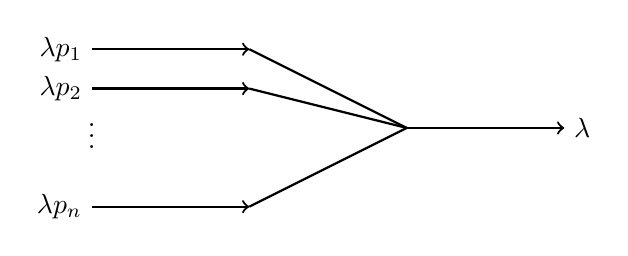
\begin{tikzpicture}
    % Draw the input arrows for each branch
    \draw[->, thick] (-4, 1.5) -- (-2, 1.5);
    \draw[->, thick] (-4, 1) -- (-2, 1);
    \draw[->, thick] (-4, -0.5) -- (-2, -0.5);

    % Labels for the input flows
    \node[left] at (-4, 1.5) {$\lambda p_1$};
    \node[left] at (-4, 1) {$\lambda p_2$};
    \node at (-4, 0.5) {$\vdots$};
    \node[left] at (-4, -0.5) {$\lambda p_n$};

    % Draw the merging point

    % Draw the branches
    \draw[thick] (-2, 1.5) -- (0, 0.5);
    \draw[thick] (-2, 1) -- (0, 0.5);
    \draw[thick] (-2, -0.5) -- (0, 0.5);

    % Draw the output arrow
    \draw[->, thick] (0, 0.5) -- (2, 0.5);
    \node[right] at (2, 0.5) {$\lambda$};
\end{tikzpicture}